L'algorithme de Dijkstra est un parcours en largeur d'un graphe \textbf{pondéré} et orienté. Il permet de calculer l'ensemble des plus courts chemins entre un sommet vers tous les autres sommets du graphe.

Pour modéliser le graphe, on utilisera une matrice d'adjacence $M$ pour laquelle $M_{ij}=w(i,j)$ et $w(i,j)$ représente le poids de l'arête de $i$ vers $j$. Lorsqu'il n'y a pas d'arc entre deux sommets, on aura $M_{ij}=\infty$.

\begin{exemple}  ~\\
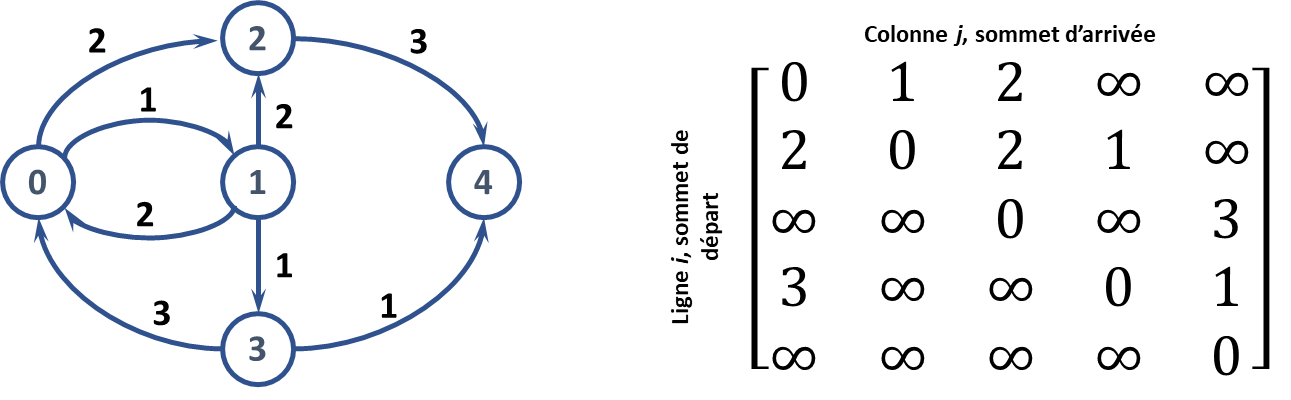
\includegraphics[width=.8\linewidth]{graphe_01}
\end{exemple}

\begin{defi}{Poids d'un chemin}
Soit un un graphe pondéré $G=\left(V, E, w\right)$ où $V$ désigne l'ensemble des sommets, $E$ l'ensemble des arêtes et 
$w$, la fonction poids définie par $w : E \rightarrow \mathbb{R}$ ($w(u, v)$ est le poids de l’arête de $u$ vers $v$).

On appelle poids du chemin $C$ et on note $w(C)$ la somme des poids des arêtes du chemin. 

Un chemin de $u\in V$ à $v\in V$ est un plus court chemin s'il n'existe pas de chemin de poids plus petit. 
\end{defi}


\begin{exemple}
Pour le chemin $C = 0, 1,2,4$, on a $w(C)=6$. 

Pour le chemin $C' = 0, 1,3,4$, on a $w(C')=3$. 

C' est un plus court chemin. 
\end{exemple}

\begin{defi} {Distance}
La distance $d\left(u,v\right)$ est le poids d'un plus court chemin de $u$ à $v$. On peut alors noter 
$d(u,v)=\inf\left\{
w(C) | C \text{ est un chemin de } u \text{ à } v
\right\}$.

Si $v$  n'est pas atteignable depuis $u$ on poser $d(u,v)=\infty$.

\end{defi}

\begin{exemple}
Dans le cas précédent, $d(0,4)=3$, 
$d(2,4)=3$ et $d(4,1)=\infty$


\end{exemple}

\begin{prop}
\textbf{Sous-optimalité} -- Soit $C$ un plus court chemin de $u$ à $v$ ainsi que $u'$ et $v'$ deux sommets de $C$. Alors le sous-chemin de $C$ de $u'$ à $v'$ est aussi un plus court chemin.
\end{prop}


\begin{exemple}
$C' = 0, 1,3,4$ est un plus court chemin; donc $C' = 1,3,4$ ou $C' = 0, 1,3$ aussi. 
\end{exemple}

\begin{obj}
Soit un graphe pondéré $G=\left(V, E, w\right)$ où $V$ désigne l'ensemble des sommets, $E$ l'ensemble des arêtes et 
$w$, la fonction poids.

Soit $s$ un sommet de $V$. L'objectif est de déterminer la liste de l'ensemble des distances entre $s$ et l'ensemble des sommets de $V$.
\end{obj}


Pour répondre à l'objectif, on peut formuler l'algorithme de Dijkstra ainsi. 


\begin{center}
\begin{tabular}{|p{1cm}p{1cm}p{1cm}p{10cm}}
\multicolumn{4}{|p{15cm}}{\textbf{Entrées : }  un graphe pondéré donné par liste ou marrice d'adjacence, un sommet \texttt{s} du graphe}\\
\multicolumn{4}{|p{15cm}}{\textbf{Sortie : } \texttt{D} liste des distances entre \texttt{s} et chacun des sommets}\\
\multicolumn{4}{|p{15cm}}{Initialisation de \texttt{D} : \texttt{D = n}$\times [\infty]$ }\\
\multicolumn{4}{|p{15cm}}{Initialisation de \texttt{D} : \texttt{D[s] =}$[0]$ }\\
\multicolumn{4}{|p{15cm}}{Initialisation de \texttt{T} : \texttt{T = n x [False] } liste des sommets traités }\\
\multicolumn{4}{|p{15cm}}{Initialisation d'une file de priorité avec le sommet de départ \texttt{F = \{s\}}}\\
\multicolumn{4}{|p{15cm}}{\textbf{Tant que} \texttt{F} n'est pas vide :  }\\
& \multicolumn{3}{|p{15cm}}{Recherche du sommet \texttt{u} tel que \texttt{d[u]} minimal parmi les sommets de \texttt{F}}\\
& \multicolumn{3}{|p{15cm}}{\textbf{Pour} tout voisin $v$ de $u$ \textbf{faire} :}\\
&& \multicolumn{2}{|p{15cm}}{\textbf{Si} $v$ n'est ni dans $T$ ni dans $F$ \textbf{alors}}\\
&&& \multicolumn{1}{|p{15cm}}{Ajouter $v$ à $F$}\\
&& \multicolumn{2}{|p{15cm}}{\texttt{D=}$\min \left(d[v],d[u]+w(u,v)\right)$}\\
& \multicolumn{3}{|p{15cm}}{\texttt{T[u] =  True}}\\
\multicolumn{4}{|p{15cm}}{Renvoyer \texttt{D}}\\
%&&& \multicolumn{1}{|p{15cm}}{}\\
%&& \multicolumn{2}{|p{15cm}}{}\\
%& \multicolumn{3}{|p{15cm}}{}\\
%\multicolumn{4}{|p{15cm}}{}\\
\end{tabular}
\end{center}

Une des étapes qui diffère avec le parcours en largeur notamment, est l'utilisation d'une file de priorité et la recherche du sommet vérifiant $d[u]$ minimal. Cela signifie que lorsqu'on partira d'un sommet \texttt{s}, on déterminera alors l'ensemble des distances permettant d'atteindre les voisins de \texttt{s}. \`A l'itération suivante, on visitera alors le sommet ayant la distance la plus faible.

\begin{defi}{File de priorité}
Une file de priorité est une structure de données sur laquelle on peut effectuer les opérations suivantes : 
\begin{itemize}
\item insérer un élement;
\item extraire l'élément ayant, dans notre cas, la plus petite valeur;
\item tester si la file de priorité est vide ou pas.
\end{itemize}

\end{defi}

\begin{exemple}
Soit une file de priorité comprenant les éléments suivants : \texttt{file = [12,1,4,5]}. La file de priorité est dotée d'une méthode \texttt{pop} permettant d'extraire la plus petite valeur. 
Ainsi, \texttt{file.pop()} renvoie \texttt{1} et la file contient alors les éléments \texttt{ [12,4,5]}. 
En réitérant \texttt{file.pop()} renverra la valeur \texttt{4} et la file contient désormais  les éléments \texttt{ [12,5]}.


Soit une file de priorité comprenant les éléments suivants : \texttt{file = [(1,2),(2,5),(0,1)]}. La méthode \texttt{pop} permetttra d'extraire le couple pour lequel la première valeur est la plus petite. 

Ainsi, \texttt{file.pop()} renvoie \texttt{(0,1)} et la file contient alors les éléments \texttt{[(1,2),(2,5)]} etc.

\end{exemple}


\begin{exemple} \textit{[Jules Svartz]} 
La figure suivante représente le déroulement de l’algorithme de Dijkstra sur un graphe à 5 sommets, depuis 
la source $s$. Pour chaque sommet $u$ on a fait figurer la valeur $d[u]$ à l’intérieur du cercle. Les arcs en gras représentent
l’évolution de la liste des prédecesseurs.

\begin{center}
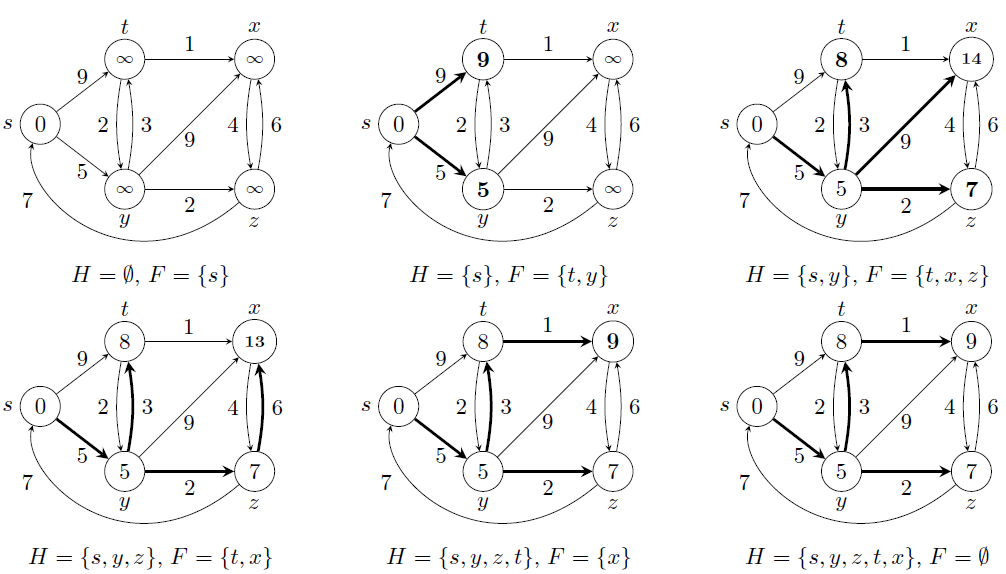
\includegraphics[width=15cm]{dijkstra}
\end{center}
\end{exemple}

On peut donc commencer par implémenter une fonction \texttt{cherche\_min} permettant de trouver le sommet \texttt{i} vérifiant \texttt{d[i]} minimal
parmi les sommets n'ayant pas été traités.% (s’il existe un tel sommet vérifiant \texttt{d[i] <}$+\infty$ , sinon $-1$ est renvoyé.


\begin{lstlisting}
def cherche_min(d, traites):
    """ Renvoie le sommet i vérifiant d[i] minimal et traites[i] faux, s'il existe un tel sommet
    tel que d[i] != inf. Sinon, renvoie -1 """
    n=len(d)
    x=-1
    for i in range(n):
        if not traites[i] and d[i] != float('inf') and (x==-1 or d[x]>d[i]):
            x=i
    return x
\end{lstlisting}


On donne alors l'algorithme de Dijkstra.

\begin{lstlisting}
def dijkstra_mat(G,s):
    """ 
    G donné par matrice d'adjacence. Renvoie les poids chemins de plus petits poids depuis s. 
    """
    n=len(G)
    d = [float('inf')]*n
    d[s]=0
    traites = [False]*n
    while True:
        x=cherche_min(d,traites)
        if x==-1:
            return d
        for i in range(n):
            d[i]=min(d[i], d[x]+G[x][i])
        traites[x]=True
\end{lstlisting}

\begin{prop}
Pour $n$ sommets et $a$ arcs, on peut montrer que, la complexité de l'algorithme est en $\mathcal{O}\left(a+n\log n\right)$.
\end{prop}

\begin{exemple}
Reprendre le graphe précédent et utiliser l'algorithme de Dijkstra en partant du sommet $t$.
\end{exemple}

%https ://www.youtube.com/watch ?v=GC-nBgi9r0U
%%https://www.youtube.com/watch?v=g024lzsknDo
\vfill
\textbf{Sources}
\begin{itemize}
\item Cours de Quentin Fortier.
\item Cours de Jules Svartz, Lycée Masséna.
\end{itemize}